\documentclass[12pt, a4paper]{mwart}

\usepackage[utf8]{inputenc}								%kodowanie znaków
\usepackage[T1]{fontenc}								%kodowanie fontu
\usepackage{polski}										%polskie wcięcia itp
\usepackage{graphicx}									%wstawianie grafik
\usepackage{booktabs}									%scalanie kolumn
\usepackage{enumitem}									%lista a), b), c)
\usepackage{multirow}									%scalanie komórek tabeli w pionie
\usepackage{listings}									%wklejanie kodu z SQL
\usepackage{xcolor}										%żeby kolory do kodu działaly
\usepackage[margin=0.5in]{geometry}						%zmiana marginesów
\usepackage[hidelinks]{hyperref}						%linki w spisie treści

\hypersetup{linktoc=all}								%ustawienie linków w spisie treści
\linespread{1.3}										%interlinia 1,5

\lstset{ %
  backgroundcolor=\color{white},   % choose the background color; you must add \usepackage{color} or \usepackage{xcolor}; should come as last argument
  basicstyle=\scriptsize,        % the size of the fonts that are used for the code
  breakatwhitespace=false,         % sets if automatic breaks should only happen at whitespace
  breaklines=true,                 % sets automatic line breaking
  commentstyle=\color{gray},       % comment style
  extendedchars=true,              % lets you use non-ASCII characters; for 8-bits encodings only, does not work with UTF-8
  frame=single,	                   % adds a frame around the code
  language=[Sharp]C,
  keywordstyle=\color{blue},       % keyword style
  morekeywords={*,...},            % if you want to add more keywords to the set
  numbers=left,                    % where to put the line-numbers; possible values are (none, left, right)
  numbersep=5pt,                   % how far the line-numbers are from the code
  numberstyle=\normalsize,			% the style that is used for the line-numbers
  rulecolor=\color{black},         % if not set, the frame-color may be changed on line-breaks within not-black text (e.g. comments (green here))
  showspaces=false,                % show spaces everywhere adding particular underscores; it overrides 'showstringspaces'
  showstringspaces=false,          % underline spaces within strings only
  showtabs=false,                  % show tabs within strings adding particular underscores
  stepnumber=1,                    % the step between two line-numbers. If it's 1, each line will be numbered
  stringstyle=\color{orange},      % string literal style
  tabsize=2	                   	   % sets default tabsize to 2 spaces                   
}

\lstset{
literate=%
{ą}{{\k{a}}}1
{Ą}{{\k{A}}}1
{ć}{{\'c}}1
{Ć}{{\'{C}}}1
{ę}{{\k{e}}}1
{Ę}{{\k{E}}}1
{ł}{{\l{}}}1
{Ł}{{\L{}}}1
{ń}{{\'n}}1
{Ń}{{\'N}}1
{ó}{{\'o}}1
{Ó}{{\'O}}1
{ś}{{\'s}}1
{Ś}{{\'S}}1
{ż}{{\.z}}1
{Ż}{{\.Z}}1
{ź}{{\'z}}1
{Ź}{{\'Z}}1
}

\begin{document}

\begin{center}
Piotr Wróbel

Entity Framework \ppauza sprawozdanie
\end{center}

\tableofcontents

\section{Wstęp}

Wykonywanie ćwiczenia na laboratorium zakończono na etapie osadzania tabeli Category na formularzu CategoryForm, ustawienia pola CategoryID jako tylko do odczytu i wykonaniu programu (punkt IVg instrukcji), stąd opis w niniejszym sprawozdaniu rozpoczęto od następnego w kolejności punktu.

\section{Bindowanie danych do komórek}

Po uruchomieniu programu na etapie punktu IVf instrukcji nie zaobserwowano ładowania danych z~tabeli do osadzonej na formularzu kontrolki. Aby to zmienić, zdefiniowano metodę Load formularza CategoryForm w~następujący sposób:

\begin{lstlisting}
private void CategoryForm_Load(object sender, EventArgs e)
{
	base.OnLoad(e);

	prodContext = new ProdContext();
	prodContext.Categories.Load();
	this.categoryBindingSource.DataSource = prodContext.Categories.Local.ToBindingList();
}
\end{lstlisting}

Po ponownym uruchomieniu programu po modyfikacji zaobserwowano poprawne ładowanie danych do kontrolki. Następnie dodano do formularza przycisk służący do zapisywania zmian i~przypisano zapisywanie danych do bazy do zdarzenia obsługującego jego kliknięcie:

\begin{lstlisting}
private void saveButton_Click(object sender, EventArgs e)
{
	prodContext.SaveChanges();

	this.categoryDataGridView.Refresh();
}
\end{lstlisting}

Poprawność działania zweryfikowano wywołując polecenie select na tabeli Categories przed i~po zapisaniu zmian w~formularzu (Rysunki~\ref{rys:4.1}\dywiz{}\ref{rys:4.4}).

\begin{figure}
  \centering
  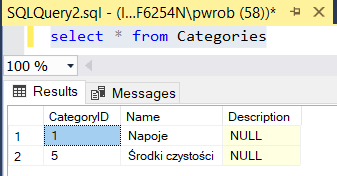
\includegraphics[scale=0.5]{IV/4-1.png}
  \caption{Stan tabeli Categories przed modyfikacją}
  \label{rys:4.1}
\end{figure}

\begin{figure}
  \centering
  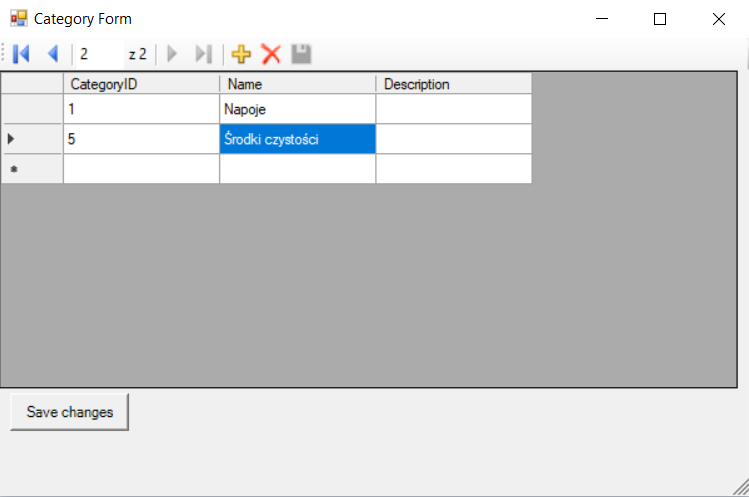
\includegraphics[scale=0.5]{IV/4-2.png}
  \caption{Formularz CategoryForm przed modyfikacją}
  \label{rys:4.2}
\end{figure}

\begin{figure}
  \centering
  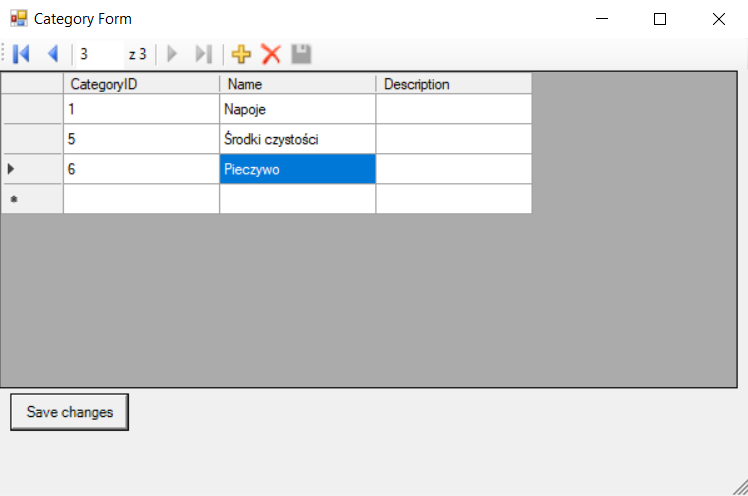
\includegraphics[scale=0.5]{IV/4-3.png}
  \caption{Formularz CategoryForm po modyfikacji}
  \label{rys:4.3}
\end{figure}

\begin{figure}
  \centering
  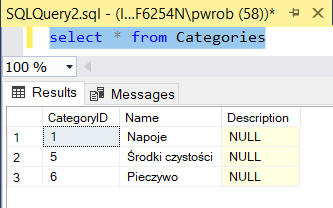
\includegraphics[scale=0.5]{IV/4-4.png}
  \caption{Po wciśnięciu przycisku Save changes zaobserwowano zapisanie zmian do bazy}
  \label{rys:4.4}
\end{figure}

W analogiczny sposób jak dla tabeli Categories, do formularza dodano kontrolkę wyświetlającą zawartość tabeli Products. W celu zapewnienia wyświetlania tylko produktów z~aktualnie zaznaczonej kategorii, a~także poprawnego działania zapisywania nowych danych do bazy (dla przefiltrowanych danych kliknięcie przycisku Save changes nie zadziałałoby), wprowadzono na formularz przycisk przełączający między trybem przeglądania i~zapisywania danych (aktualny tryb jest rozpoznawany dzięki globalnej zmiennej boolowskiej isSavingMode). Dodatkowo zmienna globalna currentCategoryID przechowuje ID aktualnie zaznaczonej kategorii. Do zdarzeń CellContentClick i~RowEnter kontrolki categoryDataGridView przypisano metodę:

\begin{lstlisting}
private void handleCategorySelection(object sender, DataGridViewCellEventArgs e)
{
	int selectedRow = e.RowIndex;
	Category selectedCategory = (Category)categoryDataGridView.Rows[selectedRow].DataBoundItem;

	if (selectedCategory != null)
	{
		currentCategoryID = selectedCategory.CategoryID;
		if (!this.isSavingMode)
		{
			// query based syntax
			this.productBindingSource.DataSource = (from prod in prodContext.Products
													where prod.CategoryID == currentCategoryID
                                                    select prod).ToList();

			// method based syntax
			//this.productBindingSource.DataSource = 
            //prodContext.Products.Where(prod => prod.CategoryID == currentCategoryID)
            //.ToList();
		}
	}
}
\end{lstlisting}

A~do zdarzenia obsługującego kliknięcie przycisku switchButton:

\begin{lstlisting}
private void switchModeButton_Click(object sender, EventArgs e)
{
	if(isSavingMode)
	{                
		this.switchModeButton.Text = "Edit mode";

		this.productBindingSource.DataSource = 
			prodContext.Products.Where(prod => prod.CategoryID == currentCategoryID).ToList();
	}
	else
	{
		this.switchModeButton.Text = "Read mode";

		productBindingSource.DataSource = prodContext.Products.Local.ToBindingList();
	}

	this.saveButton.Enabled = !this.saveButton.Enabled;

	this.productDataGridView.AllowUserToAddRows = 
		!this.productDataGridView.AllowUserToAddRows;
	this.productDataGridView.AllowUserToDeleteRows = 
		!this.productDataGridView.AllowUserToDeleteRows;

	this.categoryDataGridView.AllowUserToAddRows = 
		!this.categoryDataGridView.AllowUserToAddRows;
	this.categoryDataGridView.AllowUserToDeleteRows = 
		!this.categoryDataGridView.AllowUserToDeleteRows;

	isSavingMode = !isSavingMode;
}
\end{lstlisting}

W~celu zapewnienia poprawności dodawanych nowych danych, zaimplementowano metodę DefaultValuesNeeded kontrolki productDataGridView:

\begin{lstlisting}
private void productDataGridView_DefaultValuesNeeded(object sender, DataGridViewRowEventArgs e)
{
	e.Row.Cells["prodDGVCategoryID"].Value = currentCategoryID;
}
\end{lstlisting}

Działanie programu po dodaniu modyfikacji przedstawiono na screenach (Rysunek~\ref{rys:4.5}\dywiz{}\ref{rys:4.7}).

\begin{figure}[h]
  \centering
  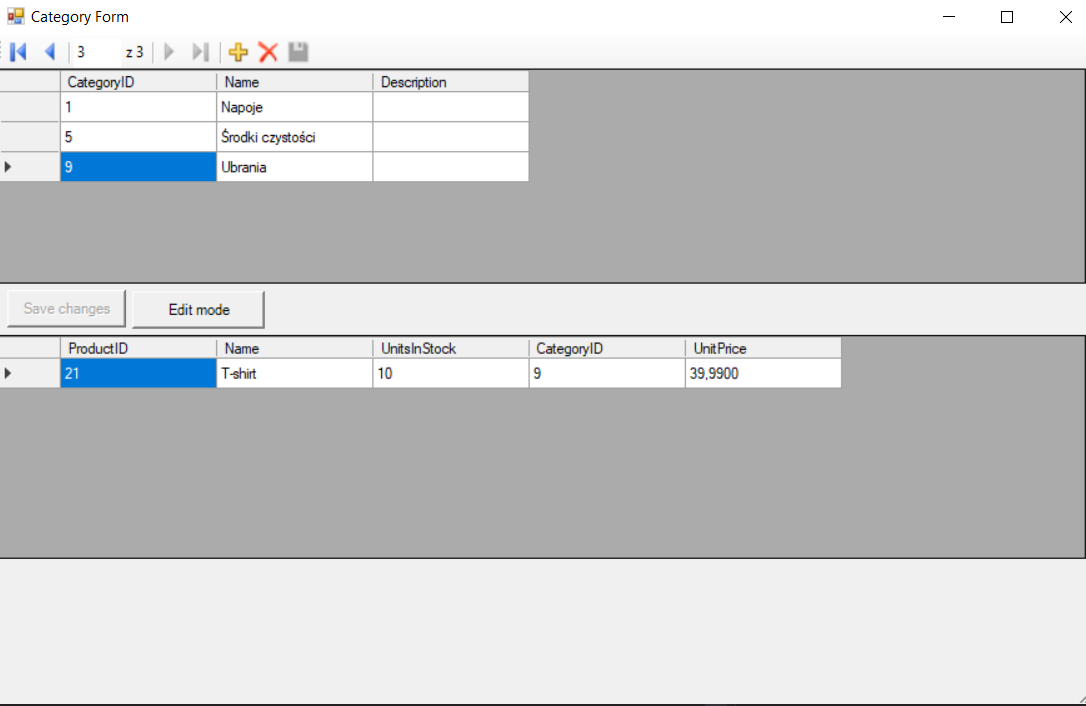
\includegraphics[scale=0.45]{IV/4-5.png}
  \caption{Tryb przeglądania danych}
  \label{rys:4.5}
\end{figure}

\begin{figure}[h]
  \centering
  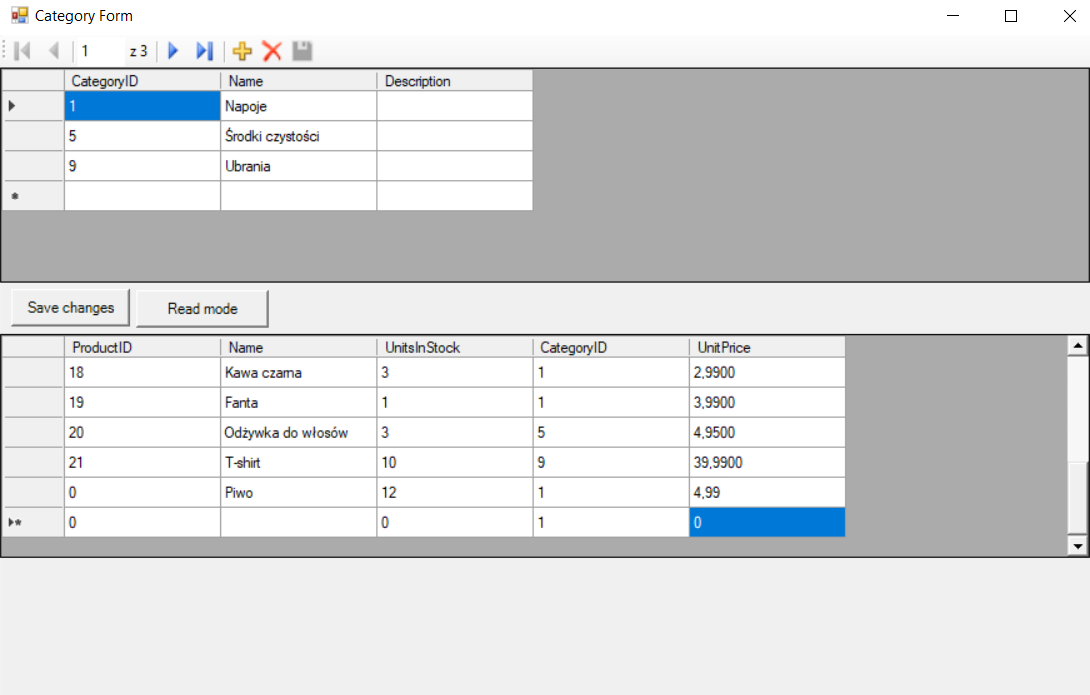
\includegraphics[scale=0.45]{IV/4-6.png}
  \caption{Tryb modyfikacji danych}
  \label{rys:4.6}
\end{figure}

\begin{figure}[ht]
  \centering
  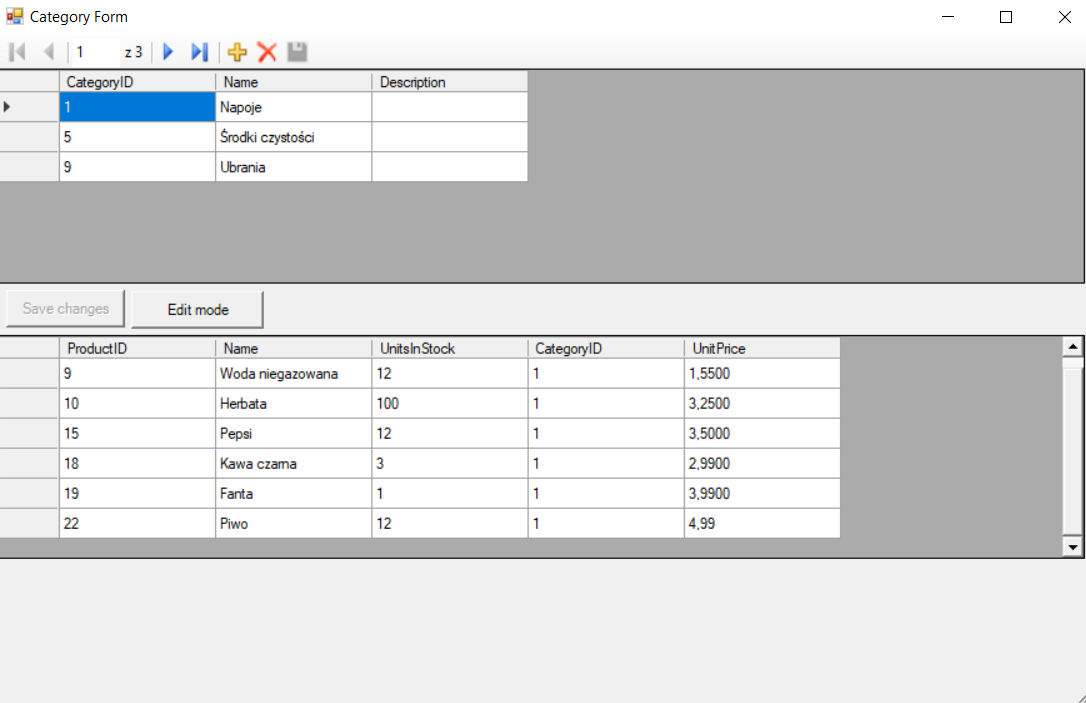
\includegraphics[scale=0.45]{IV/4-7.png}
  \caption{Po zapisaniu nowych danych i kliknięciu odpowiedniej kategorii}
  \label{rys:4.7}
\end{figure}

\section{Method syntax vs query syntax}

W~konsolowej części aplikacji zaimplementowano wypisywanie wszystkich kategorii korzystając z~method based syntax bez wymuszania automatycznej ewaluacji zapytania:

\begin{lstlisting}
// punkt V
// deferred query execution
using(ProdContext prodContext = new ProdContext())
{
	IQueryable<String> categoryNames = prodContext.Categories.Select(c => c.Name);

	Console.WriteLine("Category names:");

	foreach(String categoryName in categoryNames)
	{
		Console.WriteLine(categoryName);
	}
	Console.ReadLine();
}
\end{lstlisting}

Ustawiając odpowiednie breakpointy zaobserwowano w~SQL Server Profilerze, że zapytanie jest wykonywane dopiero w momencie wejścia do pętli foreach.

Następnie zmodyfikowano kod, tak aby zapytanie było wywoływane natychmiastowo:

\begin{lstlisting}
// immediate query execution
            
using (ProdContext prodContext = new ProdContext())
{
	List<String> categoryNames = prodContext.Categories.Select(c => c.Name).ToList();

	Console.WriteLine("Category names:");

	foreach (String categoryName in categoryNames)
	{
		Console.WriteLine(categoryName);
	}
	Console.ReadLine();
}            
\end{lstlisting}

Tym razem zaobserwowano, że zapytanie select jest wykonywane już w~momencie definicji zapytania, jeszcze przed wejściem do pętli.

Zdefiniowano funkcje wypisujące kategorie i~produkty, w~wersji query based syntax:
\begin{lstlisting}
// query based syntax - categories and products (join, lazy loading)
            
using (ProdContext prodContext = new ProdContext())
{
	IQueryable<Category> categories = prodContext.Categories;
	IQueryable<Product> products = prodContext.Products;

	var query =                    
		from category in categories
		join product in products
		on category.CategoryID equals product.CategoryID
		select new
		{
			CategoryID = category.CategoryID,
			CategoryName = category.Name,
			CategoryDescription = category.Description,
			ProductID = product.ProductID,
			ProductName = product.Name,
			UnitsInStock = product.UnitsInStock,
			UnitPrice = product.UnitPrice
		};

	foreach (var category in query)
	{
		Console.WriteLine("{0}\t{1}\t{2}\t\t\t{3}\t{4}\t{5}\t{6}",
        	category.CategoryID,
            category.CategoryName,
            category.CategoryDescription,
            category.ProductID,
            category.ProductName,
            category.UnitsInStock,
            category.UnitPrice
		);
	}
	Console.Read();
}
\end{lstlisting}

i~w~wersji method based syntax:
\begin{lstlisting}
// method based syntax (navigation property, eager loading)

using (ProdContext prodContext = new ProdContext())
{
	var categoryQuery = prodContext.Categories.Include("Product").Select(cat => new
	{
		CategoryID = cat.CategoryID,
		CategoryName = cat.Name,
		CategoryDescription = cat.Description,
		CategoryProducts = cat.Products
	});

	foreach (var category in categoryQuery)
	{
		Console.WriteLine("{0}\t{1}\t{2}",
			category.CategoryID,
			category.CategoryName,
			category.CategoryDescription
		);
		foreach (Product product in category.CategoryProducts)
		{
			Console.WriteLine("\t\t\t\t{0}\t{1}\t{2}\t{3}",
				product.ProductID,
				product.Name,
				product.UnitsInStock,
				product.UnitPrice);
		}
	}
	Console.Read();
}            
\end{lstlisting}

Ponadto zaimplementowano funkcję zliczającą ilość produktów w~poszczególnych kategoriach, w~wersji query based syntax:
\begin{lstlisting}
// products number
// query based syntax (lazy loading)

using (ProdContext prodContext = new ProdContext())
{
	var query = from category in prodContext.Categories
		select new
		{
			CategoryID = category.CategoryID,
			Name = category.Name,
			Description = category.Description,
			ProdCount = category.Products.Count()
		};

	foreach (var category in query)
	{
		Console.WriteLine("{0}\t{1}\t{2}\t{3}",
			category.CategoryID,
			category.Name,
			category.Description,
			category.ProdCount);
	}
	Console.Read();
}
\end{lstlisting}

i~w~wersji method based syntax:
\begin{lstlisting}
// method based syntax (navigation property, lazy loading)

using (ProdContext prodContext = new ProdContext())
{
	var categoryQuery = prodContext.Categories.Include("Product").Select(cat => new
	{
		CategoryID = cat.CategoryID,
		CategoryName = cat.Name,
		CategoryDescription = cat.Description,
		CategoryProducts = cat.Products
	});

	foreach (var category in categoryQuery)
	{
		int productsCount = 0;
		foreach (Product product in category.CategoryProducts)
		{
			productsCount++;
		}

		Console.WriteLine("{0}\t{1}\t{2}\t{3}",
			category.CategoryID,
			category.CategoryName,
			category.CategoryDescription,
			productsCount);
	}

	Console.Read();
}
\end{lstlisting}

\section{Zadanie domowe}

Aby możliwe było złożenie zamówienia przez konkretnego użytkownika, dodano nowy formularz służący do logowania (podania nazwy użytkownika znajdującej się w~bazie) \ppauza Rysunek~\ref{rys:6.1}. 

\begin{figure}[ht]
  \centering
  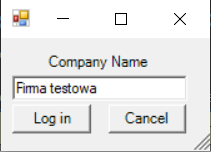
\includegraphics[scale=1.0]{VI/6-1.png}
  \caption{Formularz logowania}
  \label{rys:6.1}
\end{figure}

Jeżeli podano nazwę znajdującą się w~tabeli Customers, to otwierany jest formularz zamówienia (odpowiednio rozbudowany w~stosunku do punktu IV), kod odpowiedzialny za sprawdzanie zgodności nazwy został przypisany do obsługi kliknięcia przycisku Log in. Ponadto do formularza CategoryForm dodano atrybut będący nazwą zalogowanego użytkownika przekazywany w~konstruktorze.

\begin{lstlisting}
private void loginButton_Click(object sender, EventArgs e)
{
	String companyName = this.companyNameTextBox.Text;
	bool companyExists = prodContext.Customers.Any(c => c.CompanyName == companyName);

	if(!companyExists)
	{
		MessageBox.Show("Non-valid company name", "Logging error", MessageBoxButtons.OK);
	}
	else
	{
		CategoryForm categoryForm = new CategoryForm(companyName);
		categoryForm.ShowDialog();
		this.Close();
	}
}
\end{lstlisting}

W aplikacji istnieje specjalny użytkownik Admin, który ma możliwość modyfikacji pól dotyczących produktów i~kategorii. Kwestia, czy bieżącemu użytkownikowi można przypisać takie uprawnienia, jest sprawdzana przy ładowaniu CategoryForm:

\begin{lstlisting}
if (companyName == "Admin")
{
	this.saveButton.Enabled = false;
	this.switchModeButton.Text = "Edit mode";
}
else
{
	this.saveButton.Visible = false;
	this.switchModeButton.Visible = false;                               
}
\end{lstlisting}

Do obsługi zamówień, dodano nową klasę Order:
\begin{lstlisting}
public class Order
{
	public int OrderID { get; set; }
	[ForeignKey("Product")]
	public int ProductID { get; set; }

	[Required]
	public int NumberOfUnits { get; set; }

	[ForeignKey("Customer")]
	public String CompanyName { get; set; }
	public virtual Customer Customer { get; set; }
	public virtual Product Product { get; set; }
}
\end{lstlisting}

Zmodyfikowano formularz CategoryForm, dodając do niego pola służące do dodawania i usuwania pozycji do/z zamówienia. Ponadto umieszczono etykietę zawierającą całkowitą wartość zamówienia, a~także przyciski Order \ppauza zapisujący dane zamówienia do bazy i~Cancel \ppauza czyszczący wszystkie dane o zamówieniu z formularza. Nowy wygląd formularza przedstawia Rysunek~\ref{rys:6.2}.

\begin{figure}[ht]
  \centering
  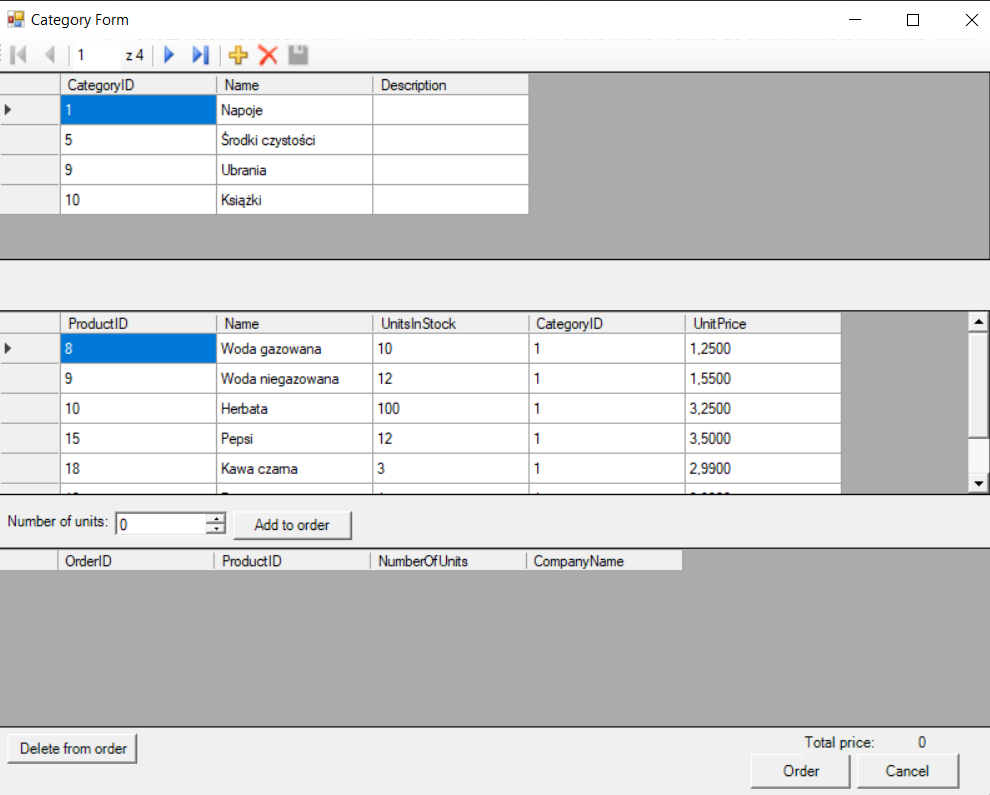
\includegraphics[scale=0.5]{VI/6-2.png}
  \caption{Formularz zamawiania}
  \label{rys:6.2}
\end{figure}

O~ile w~bazie na etapie ładowania formularza istnieją jakieś wpisy w~tabeli Order, to przy jego ładowaniu jest sumowana wartość wszystkich produktów z~wykorzystaniem NavigationProperty:

\begin{lstlisting}
this.orderBindingSource.DataSource = prodContext.Orders.Local.Where(ord => 
	ord.CompanyName == companyName).ToList();
this.totalPrice = 0;

foreach (Order order in (List<Order>) orderBindingSource.DataSource)
{
	Product currentProduct = order.Product;
	this.totalPrice += currentProduct.UnitPrice * order.NumberOfUnits;
}

this.totalPriceLabel.Text = Convert.ToString(this.totalPrice);
\end{lstlisting}

Przy dodawaniu pozycji do zamówienia sprawdzane jest czy podana ilość jest niezerowa (mniejsze wartości są wykluczone na etapie odpowiedniego ustawienia kontrolki) oraz czy nie przekracza ilości zadeklarowanej w~tabeli Products. W~przeciwnym wypadku tworzona jest nowa pozycja zamówienia, dodawana do kontekstu oraz pomniejszana jest dostępna ilość w~tabeli Products, a~także aktualizowana zawartość etykiety wyświetlającej cenę:

\begin{lstlisting}
private void addToOrderButton_Click(object sender, EventArgs e)
{
    int selectedProductRowIndex = productDataGridView.SelectedCells[0].RowIndex;
    DataGridViewRow selectedProductRow = productDataGridView.Rows[selectedProductRowIndex];
    int maxUnits = Convert.ToInt32(selectedProductRow.Cells["prodDGVUnitsInStock"].Value);

    if(this.numberOfUnitsUpDown.Value == 0 || this.numberOfUnitsUpDown.Value > maxUnits)
    {
    	MessageBox.Show("Incorrect unit number!", "Error", MessageBoxButtons.OK);
    }
    else
    {
		Order newOrder = new Order();
		newOrder.CompanyName = this.companyName;
		newOrder.NumberOfUnits = (int) this.numberOfUnitsUpDown.Value;
		newOrder.ProductID = Convert.ToInt32(selectedProductRow.Cells["prodDGVProductID"].Value);
		prodContext.Orders.Add(newOrder);

		orderBindingSource.DataSource = prodContext.Orders.Local.Where(ord => 
			ord.CompanyName == companyName).ToList();               

		Product productToModify = prodContext.Products.First(prod => 
			prod.ProductID == newOrder.ProductID);
		productToModify.UnitsInStock -= newOrder.NumberOfUnits;
		productDataGridView.Refresh();

		this.totalPrice += productToModify.UnitPrice * newOrder.NumberOfUnits;
		this.totalPriceLabel.Text = Convert.ToString(this.totalPrice);
	}
}
\end{lstlisting}

Analogicznie zaimplementowano usuwanie pozycji z~zamówienia:

\begin{lstlisting}
private void deleteFromOrder_Click(object sender, EventArgs e)
{
    int selectedOrderRowIndex = orderDataGridView.SelectedCells[0].RowIndex;
    DataGridViewRow selectedOrderRow = orderDataGridView.Rows[selectedOrderRowIndex];
    int productToChangeID = Convert.ToInt32(selectedOrderRow.Cells["orderDGVProductID"].Value);
    int cancelledUnits = Convert.ToInt32(selectedOrderRow.Cells["orderDGVNumberOfUnits"].Value);
    int cancelledOrderID = Convert.ToInt32(selectedOrderRow.Cells["orderDGVOrderID"].Value);

    Order orderToRemove = prodContext.Orders.Local.First(ord => 
    	(ord.ProductID == productToChangeID)  &&
    	((ord.ProductID == productToChangeID) &&
    	(ord.NumberOfUnits == cancelledUnits) &&
    	(String.Compare(ord.CompanyName, this.companyName) == 0)));
            
    Product productToModify = prodContext.Products.First(prod => prod.ProductID == productToChangeID);
    productToModify.UnitsInStock += cancelledUnits;
    productDataGridView.Refresh();

    this.totalPrice -= cancelledUnits * productToModify.UnitPrice;
    this.totalPriceLabel.Text = Convert.ToString(this.totalPrice);

    prodContext.Orders.Local.Remove(orderToRemove);
    orderBindingSource.DataSource = prodContext.Orders.Local.Where(ord => 
		ord.CompanyName == companyName).ToList();
}
\end{lstlisting}

Przykładowe działanie przedstawiono na Rysunkach~\ref{rys:6.3}\dywiz{}\ref{rys:6.5}.

\begin{figure}[ht]
  \centering
  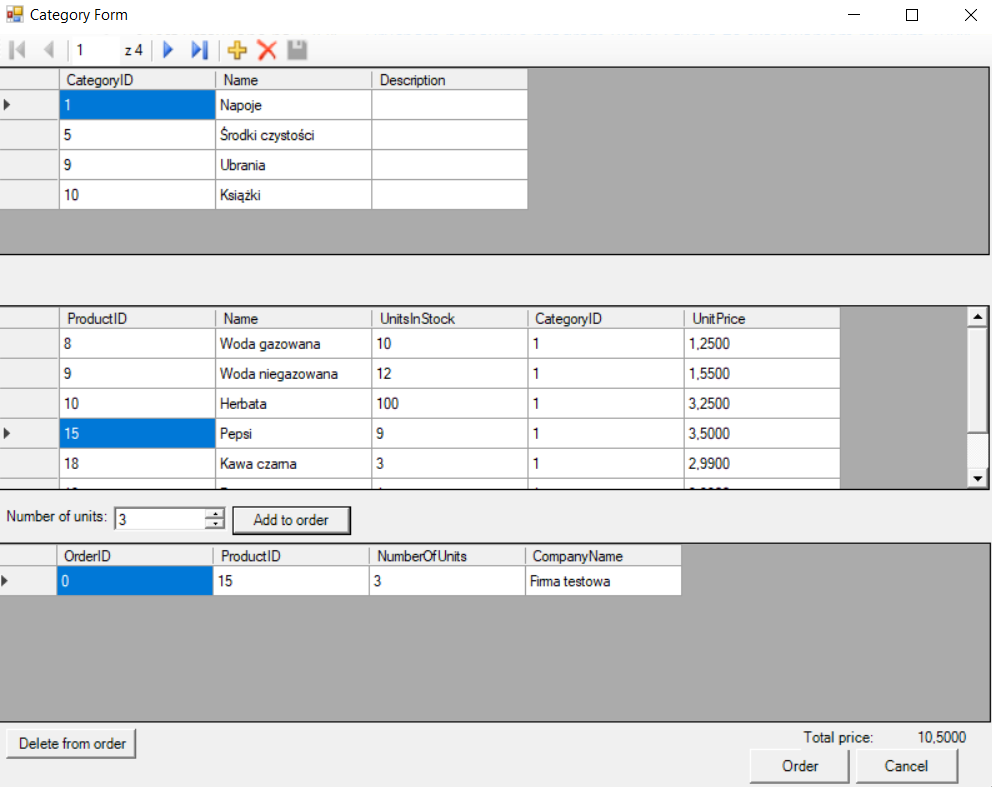
\includegraphics[scale=0.5]{VI/6-3.png}
  \caption{Dodanie nowego zamówienia}
  \label{rys:6.3}
\end{figure}

\begin{figure}[ht]
  \centering
  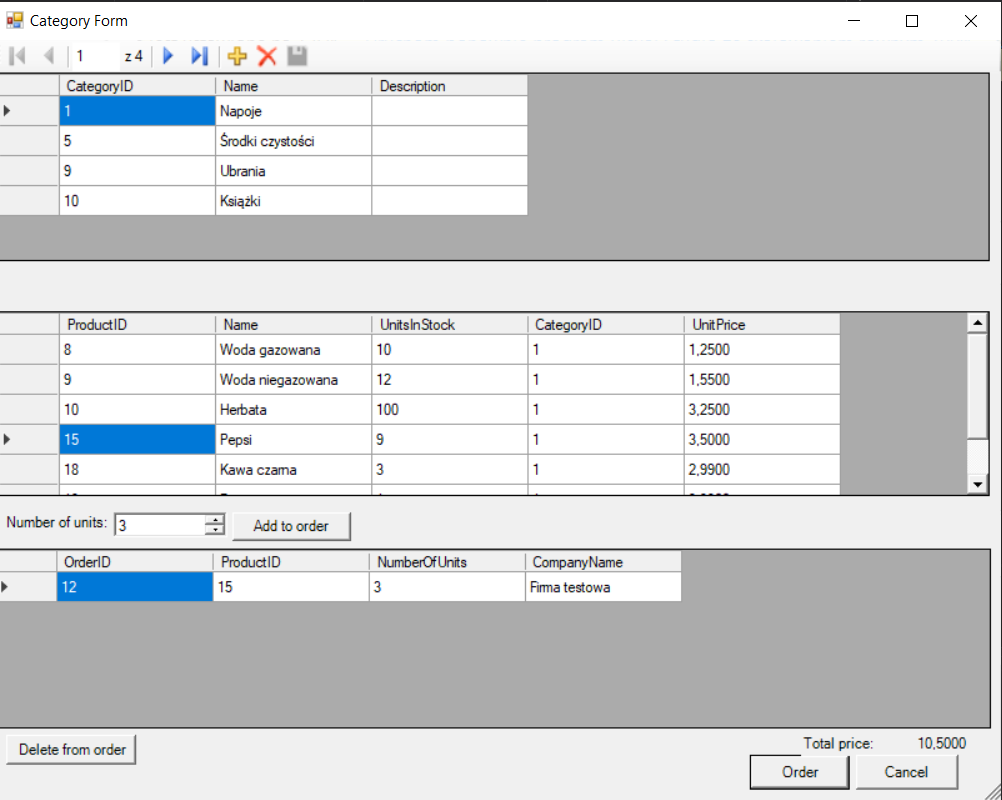
\includegraphics[scale=0.5]{VI/6-4.png}
  \caption{Zapisanie zmian w~kontekście}
  \label{rys:6.4}
\end{figure}

\begin{figure}[ht]
  \centering
  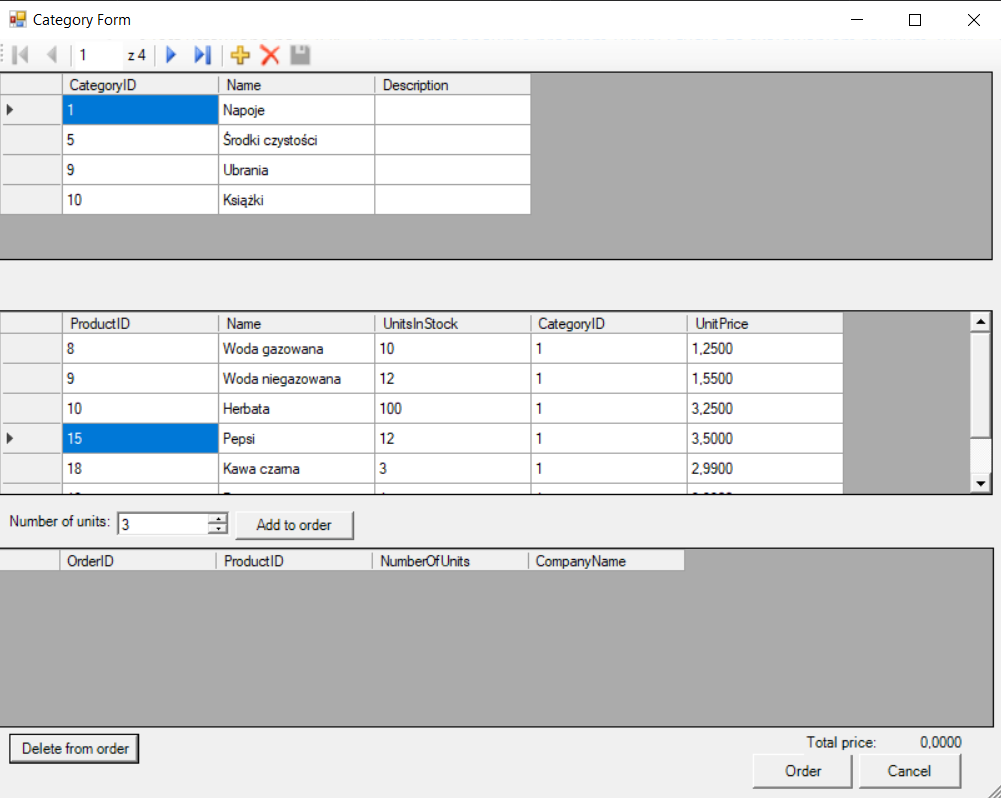
\includegraphics[scale=0.5]{VI/6-5.png}
  \caption{Usuwanie zamówienia}
  \label{rys:6.5}
\end{figure}

\end{document}